\documentclass[a4paper,12pt]{article}
\usepackage[sorting=none]{biblatex}
\usepackage[portuguese]{babel}
\usepackage[none]{hyphenat}
\usepackage{graphicx}

\usepackage{courier} %% Sets font for listing as Courier.
\usepackage{listings, xcolor}
\lstset{
tabsize = 4, %% set tab space width
showstringspaces = false, %% prevent space marking in strings, string is defined as the text that is generally printed directly to the console
numbers = left, %% display line numbers on the left
commentstyle = \color{olive}, %% set comment color
keywordstyle = \color{blue}, %% set keyword color
stringstyle = \color{red}, %% set string color
rulecolor = \color{black}, %% set frame color to avoid being affected by text color
basicstyle = \small \ttfamily , %% set listing font and size
breaklines = true, %% enable line breaking
numberstyle = \tiny,
}

\addbibresource{references.bib}
% pdflatex

% redefines the page margins
\setlength{\textheight}{24.00cm}
\setlength{\textwidth}{15.50cm}
\setlength{\topmargin}{0.35cm}
\setlength{\headheight}{0cm}
\setlength{\headsep}{0cm}
\setlength{\oddsidemargin}{0.25cm}

\makeatletter
\renewcommand\paragraph{\@startsection{paragraph}{4}{\z@}%
                {-3.25ex\@plus -1ex \@minus -.2ex}%
                {1.5ex \@plus .2ex}%
                {\normalfont\normalsize\bfseries}}
\renewcommand\subparagraph{\@startsection{subparagraph}{5}{\z@}%
                {-3.25ex\@plus -1ex \@minus -.2ex}%
                {1.5ex \@plus .2ex}%
                {\normalfont\normalsize\bfseries}}
\makeatother
\setcounter{secnumdepth}{5} % how many sectioning levels to assign numbers to
\setcounter{tocdepth}{5}    % how many sectioning levels to show in ToC

\begin{document}

\begin{titlepage}
% \pagecolor{blue!10}
\begin{center}

\textsc{\Large \textcolor{black}{\textbf{Instituto Superior de Engenharia de Lisboa}}}\\[0.4cm]	

{\huge \Large{Departamento de Engenharia Eletrónica e de Computadores} \\[1cm] }


\includegraphics{logoISEL}\\[1cm]

\textsc{\Large \textbf{Relatório Final}}\\[0.4cm]	


%%% Título
\rule{\linewidth}{0.7mm} \\[0.4cm]
{ \Large \bfseries\color{black!70!black} Inteligência Artificial para Sistemas Autónomos \\[0.4cm] }
\rule{\linewidth}{0.7mm} \\[1cm]


\color{black!80!black}{\large \textbf{Docente:}}\\[0.6cm]

\begin{tabular}{l}
\large  Luis Morgado \\[1cm]
\end{tabular}

\color{black!80!black}{\large \textbf{Aluno:}}\\[0.6cm]
\color{black}
\centering
\begin{tabular}{l}

\large Ricardo Pinto N.º 47673 \\[0.4cm]
\end{tabular}

\vfill

% Pie de página
\large \color{black!80!black}{\textbf{junho de 2024}}\\[0.2cm]

\end{center}
\end{titlepage}

\newpage
\tableofcontents

\newpage
\listoffigures
\listoftables

\newpage
\section{Introdução}
Este relatório detalha um estudo abrangente e a implementação subsequente de um projeto que se encontra na intersecção entre a inteligência artificial para sistemas autónomos (IASA) e engenharia de software. 
O documento inicia com um enquadramento teórico sólido que visa oferecer uma visão clara sobre os conceitos fundamentais de I.A., especialmente focados no desenvolvimento de agentes reativos, e as práticas essenciais da engenharia de software que sustentam a construção de softwares robustos e eficientes.

Foram realizadas duas partes do projecto, sendo estas:
\begin{description}
	\item[Parte 1] - Agente reactivo em Java. Desenvolvido o agente e ambiente. O agente atua sobre o ambiente de um jogo, onde o objectivo é fotografar animais.
	\item[Parte 2] - Biblioteca para desenvolvimento de agentes reactivos em Python. Modulação de um agente reactivo para encontrar alvos e evitar paredes.
\end{description}
\newpage
\section{Enquadramento teórico}
\subsection{Inteligência Artificial}
A inteligência artificial é uma área científica que estuda o desenvolvimento de sistemas computacionais capazes de comportamento inteligente, que adopta duas principais perpectivas: analítica e sintética.
\begin{description}
	\item[Analítica] - por via empírica (baseada na prática, com experiências e observações) desenvolver modelos e teorias para explicar os fenómenos observados e reproduzir esses fenómenos e sistemas artificiais (dispositivos criados para o efeito).
	\item[Sintética] - com base nesses modelos e teorias, desenvolver sistemas capazes de apresentar características e comportamentos associados ao conceito de inteligência.
\end{description}

Existem 3 principais paradigmas da inteligência artificial, sendo eles:
\begin{itemize}
	\item Simbólico
	\item Conexionista
	\item Comportamental
\end{itemize}

\subsubsection{Paradigma Simbólico}
Um símbolo é um elemento discreto de representação de informação. Estes são centrais no processamento de informação e na representação de conceitos relacionados com o domínio de um problema sob a forma de estruturas simbólicas.
Neste paradigma, a inteligência é o resultado da acção de processos computacionais sobre estruturas simbólicas.

É importante notar que os símbolos não têm um significado intrínseco. O seu significado deriva das relações entre estruturas simbólicas bem como das relações dessas estruturas com as entradas e saídas do sistema. Esta relação é chamada de ancoragem simbólica, pois o significado é ancorado nas observações e conceitos referenciados.

Num sistema artificial o significado é construído através de relacionamentos entre simbolos.

\subsubsection{Paradigma Conexionista}
A inteligência é uma propriedade emergente das interacções de um número elevado de unidades elementares de processamento interligadas entre si.
Neste paradigma o processamento de informação é baseado em redes de unidades de processamento elementares (designadas neurónios) interligadas entre si, sendo a informação mantida e processada nessas redes de forma distribuída, em particular nas ligações entre neurónios, em vez de símbolos. Este paradigma é inspirado no conhecimento atual do funcionamento do cérebro humano.

\subsubsection{Paradigma Comportamental}
A inteligência resulta do comportamento individual e conjunto de múltiplos sistemas a diferentes escalas de organização tendo por base relações entre estímulos e respostas.
No paradigma comportamental o processamento de informação é baseado em relações entre estímulos e respostas, modeladas sob a forma de reacções e de comportamentos (conjuntos estruturados de reacções).

\subsubsection{Agente Inteligente}
Um sistema autónomo descreve-se pela independência, ou seja, pela capacidade de existir e funcionar sem depender de outros sistemas.

Um sistema inteligente descreve-se por possuir cognição e racionalidade.

\begin{description}
	\item[Cognição] - É o processo pelo qual um sistema adquire, processa, armaneza e utiliza informação.
	\item[Racionalidade] - É a capacidade de decidir no sentido de conseguir o melhor resultado possível perante os objectivos que se pretende obter. Ou seja, um sistema racional escolhe a acção que maximiza o valor esperado da medida de desempenho dado o conhecimento disponível sobre o ambiente, percepções e acções.
\end{description}

É de notar que para um sistema ser autónomo, este não necessita de ser inteligente, mas um sistema inteligente implica que seja também autónomo, visto que a autonomia é uma característica da inteligência.

Um sistema autónomo inteligente opera num ciclo realimentado percepção-processamento-acção, através do qual é realizado o controlo da função do sistema de modo a concretizar a finalidade desse sistema.

Um agente inteligente é a representação computacional de um sistema autónomo inteligente. Este segue o mesmo ciclo de percepção-processamento-acção. A percepção é feita através de sensores ligados ao ambiente, e a acção é feita sobre actuadores ligados ao ambiente.

Um agente inteligente pode ter as seguintes características, dependendo da sua arquitetura:
\begin{description}
	\item[Autonomia] - Capacidade de um sistema operar por si próprio, de modo independente de outros sistemas.
	\item[Reactividade] - Capacidade de reagir sobre estímulos do ambiente.
	\item[Pró-Actividade] - Capacidade de atuar sobre o ambiente, independente dos estímulos.
	\item[Sociabilidade] - Capacidade de comunicar com outros agentes, de forma a concretizar objectivos individuais ou comuns a outros agentes.
\end{description}
Estas características estão associadas à concretização da finalidade do agente, ou seja, do seu objectivo, expresso na função que realiza.

\subsubsection{Representação do Ambiente}
A representação do ambiente é um elemento de suporte do processamento interno em alguns modelos de agente inteligente.
Essas representações podem ter diferentes níveis de complexidade.

Um ambiente tem diversas propriedades:
\begin{description}
	\item[Discreto/Contínuo] - Se for discreto (como no caso de um ambiente virtual), este acontece num tempo não contínuo, ou seja, os seus pontos de informação têm um intervalo temporal. Se for contínuo (como no caso de um ambiente real), este acontece num tempo contínuo, ou seja, existem infinitos pontos de informação.
	\item[Determinístico/Estocástico] - Se for determinístico, o ambiente opera sempre da mesma forma, ou seja, cada acção leva a um resultado expectável. Se for estocástico, o ambiente opera de forma aleatória, ou seja, mesmo sabendo toda a informação do ambiente, não é possivel determinar qual será o resultado de uma acção sobre este.
	\item[Estático/Dinâmico] - Um ambiente estático não varia, enquanto que um ambiente dinâmico varia.
	\item[Totalmente/Parcialmente observável] - Se um ambiente for totalmente observável, um agente poderá ter toda a informação contida no ambiente. Se o ambiente for apenas parcialmente observável, apenas parte da informação do ambiente está disponível para o agente.
	\item[Agente único/Múltiplos agentes] - Um ambiente poderá ter apenas um agente a atuar sobre este, um vários.
\end{description}

\subsubsection{Raciocínio Automático}

O raciocínio automático refere-se à capacidade de resolver de forma automática um problema, tendo como base uma representação de conhecimento do domínio do mesmo, produzindo uma solução a partir da exploração das diversas alternativas possíveis.

Para conseguir produzir uma solução, o processo de raciocínio automático envolve 2 tipos de atividades principais, sendo estas a exploração de opções possíveis e a avaliação das opções para decidir qual a melhor.

\begin{description}
	\item[Exploração de opções possíveis] - Deve usar um raciocínio prospectivo, ou seja, deve antecipar o que pode acontecer, e requer uma simulação interna do domínio do problema.
	\item[Avaliação de opções] - As opções são avaliadas através do seu o custo, ou seja, os recursos necessários para a opção, e o seu valor, ou seja, os ganhos ou perdas da opção, que podem ser medidos, por exemplo, em termos de utilidade.
\end{description}

A representação do conhecimento do domínio do problema implica que haja uma conversão da informação concreta do problema, para estruturas simbólicas que servem como base à simulação para exploração e avaliação das opções possíveis.

Esta conversão envolve 2 processos: codificação e descodificação.
A codificação trata-se da conversão da informação concreta do problema em estruturas simbólicas internas, enquanto que a descodificação é a operação inversa, ou seja, converte as estruturas simbólicas em informações concretas do problema.

Sendo necessário guardar estruturas simbólicas para realizar a exploração de opções, é necessário estabelecer como é que estas funcionam.
Estas estruturas devem ter a informação necessária para resolver o problema, e são designadas de ''modelo do problema''. O modelo do problema é representado através de:

\begin{description}
	\item[Estado] - Representa uma configuração possível do problema. É único para um problema.
	\item[Operador] - Representa uma acção que produz uma transformação do estado. Ao operar sobre um estado, é produzida uma transição que corresponde à geração de um novo estado.
\end{description}

Tendo esta informação, é possível descrever o raciocínio automático como tendo 4 requisitos:

\begin{description}
	\item[Definição de Estado]
	\item[Definição dos Operadores]
	\item[Descrição do Problema] - Um problema pode ser descrito através de 3 elementos:\hfill \\
		Estado inicial \hfill \\
		Operadores \hfill \\
		Objectivos
	\item[Mecanismo de Raciocínio] - Mecanismo que faz a exploração e avaliação das opções possíveis, usando como base a descrição do problema, e que mantém um modelo do problema interno.
\end{description}

Um espaço de estados é um conjunto de estados e de transições de estado representado sob a forma de um grafo, onde cada vértice corresponde a um estado e cada aresta corresponde a uma transição entre estados.
\begin{figure}[h]
\centering
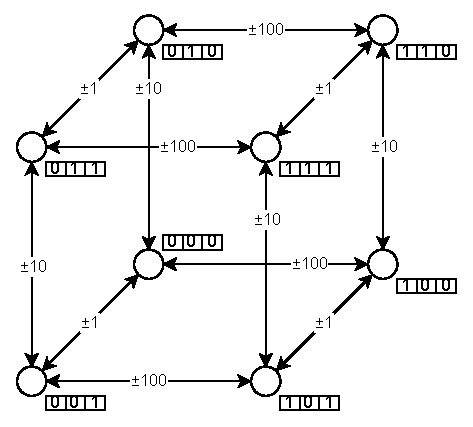
\includegraphics{espaco_estados}
\caption{Exemplo de um espaço de estados, onde o problema corresponde à contagem de um número binário com 3 casas (ou seja, de 0 a 7), onde é possível incrementar/decrementar 1, 2 ou 4.}
\end{figure}

\subsubsection{Procura em Espaços de Estados}
A procura em espaços de estados é um método de resolução de problemas de planeamento, onde se pretende encontrar uma sequência de estados e operadores que levem de um estado inicial a um estado final (estado objectivo).
Uma solução deste tipo de problemas é um percurso no espaço de estados, que liga o estado inicial a um estado objectivo.

O processo de procura ocorre por exploração do espaço de estados a partir do estado inicial. Esta exploração ocorre da seguinte forma:

Em cada passo do processamento, ocorre o seguinte:
\begin{itemize}
	\item Primeiro é verificado se o estado atual é um estado objectivo. Caso seja, o processamento termina e é retornado o percurso do estado inicial ao estado atual. Caso não seja, continua o processamento.
	\item O estado atual é expandido, sendo gerados todos os estados sucessores por aplicação de todos os operadores possíveis.
	\item É processado cada estado sucessor.
	\item Se não existiram mais estados sucessores, o processo de procura termina, não existindo solução.
\end{itemize}

Para guardar a informação gerada em cada passo da procura, é mantida uma árvore de procura quem mantém a informação relativa a cada transição de estado explorada.
Esta árvore relaciona cada nó com o seu antecessor, e mantém a informação do estado correspondente a cada nó, e o operador que originou a transição do estado antecessor para o estado do nó.

É importante conhecer alguns conceitos sobre a exploração em árvores de procura:
\begin{description}
	\item[Raiz da árvore] - Nó correspondente ao estado inicial.
	\item[Fronteira de exploração] - Estrutura de dados com relação de ordem que mantém os nós a explorar. O critério de ordenação da fronteira é o que determina a estratégia de controlo de procura.
	\item[Nó fechado] - Nó que já foi expandido.
	\item[Nó aberto] - Nó por expandir.
\end{description}

\paragraph{Métodos de procura}
Existem vários métodos de executar a procura no espaço de estados. Alguns dos aspectos a considerar para cada método de procura são:

\begin{description}
	\item[Completo] - Método que garante que, caso exista uma solução, esta é encontrada.
	\item[Óptimo] - Método que, existindo várias soluções, garante que encontra a melhor.
	\item[Complexidade Espacial] - Memória necessária para encontrar uma solução.
	\item[Complexidade Temporal] - Tempo necessário para encontrar uma solução.
\end{description}

Além disso, é necessário conhecer também os parâmetros de caracterização de um método de procura:
\begin{description}
	\item[Factor de Ramificação (Branching Factor)] - Número máximo de sucessores para um qualquer estado. Designado pela letra ''b''.
	\item[Profundidade da Procura (Search Depth)] - Profundidade do nó objectivo menos profundo da árvore de procura, ou seja, a dimensão do percurso entre o estado inicial e esse estado objectivo. Designado pela letra ''d''.
\end{description}

\subparagraph{Procura geral em grafos}
Todos os métodos de procura estudados são métodos de procura em grafos, mais concretamento, procuras no grafo do espaço de estados.

Neste tipo de procuras, é necessário eliminar os nós correspondentes a estados repetidos, e para este efeito, é necessário verificar se um novo nó sucessor corresponde a um estado que já foi previamente explorado, e se for, apenas o nó com o menor custo deve ser mantido, e os outros eliminados.

Para esta verificação, é preciso ter em conta tanto os nós abertos, como os fechados.

De modo a facilitar o processamento de nós repetidos, pode ser mantida uma única memória de nós previamentes explorados, que inclui ambos os nós abertos e os nós fechados. É importante notar que apesar de esta estrutura manter uma coleção dos nós abertos, esta não substitui a fronteira de exploração, servindo apenas para facilitar o processamento de nós repetidos.

Para um processamento mais eficiente, esta memória deve ser indexada por estado, para que haja um acesso eficiente na verificação dos nós já explorados.

\subparagraph{Procura em profundidade (Depth-First Search)}
Na procura em profundidade, o critério de exploração é a maior profundidade, ou seja, os nós mais recentes são explorados primeiro (os primeiros nós da fronteira), e os nós gerados são inseridos no início da fronteira. Isto representa uma fronteira do tipo LIFO (Last In, First Out), ou seja, onde o último nó a ser gerado é o primeiro a ser explorado.

Esta procura maximiza a profundidade do ramo corrente de procura, apenas mudando de ramo quando não for possível gerar mais estados sucessores para o estado atual.

Este tipo de procura ocupa menos memória que a procura por largura, mas não é nem óptima nem completa.
\\

Complexidade Temporal: \(O(b^m)\)
\\

Complexidade Espacial: \( O(b*m)\)
\begin{description}
	\item[b] - factor de ramificação.
	\item[m] - profundidade máxima da árvore de procura.
\end{description}

Esta procura tem 2 sub-tipos:
\begin{description}
	\item[Pocura em profundidade limitada (Depth-Limited Search)] - Procura em profundidade que limita a procura a uma profundidade máxima.
	\item[Pocura em profundidade iterativa (Iterative Deepening Search)] - Procura que realiza sucessivas procuras em profundidade limitada, com uma profundidade máxima iterativamente crescente.
\end{description}

\subparagraph{Procura em largura (Breadth-First Search)}
Na procura em largura, o critério de exploração é a menor profundidade, ou seja, os nós mais antigos são explorados primeiro (os últimos nós da fronteira), e os nós gerados são inseridos no fim da fronteira. Isto representa uma fronteira do tipo FIFO (First In, First Out), ou seja, onde o primeiro nó a ser gerado é o primeiro a ser explorado.

Esta procura explora exaustivamente cada nível de procura antes de explorar um nó a um nível de maior profundidade, apenas aumentando a profundidade quando não por possível gerar mais nós na profundidade atual.

Este tipo de procura ocupa mais memória que a procura por profundidade, mas em contra-partida, é óptima e completa.
\\

Complexidade Temporal: \(O(b^d)\)
\\

Complexidade Espacial: \( O(b*d)\)
\begin{description}
	\item[b] - factor de ramificação.
	\item[d] - dimensão da solução.
\end{description}

\subparagraph{Procura melhor-primeiro (Best-First)}
Na procura melhor-primeiro,existe uma função f(n) que é capaz de avaliar um nó, dando a este uma prioridade. Através dessa avaliação, a fronteira de exploração é ordenada por ordem crescente da prioridade de cada nó.

Tipicamente, f(n) corresponde a uma estimativa do custo da solução através do nó. Ou seja, quanto menor o valor de f(n), mais promissor é o nó.

\subparagraph{Procura de custo uniforme}
A procura de custo uniforme trata-se de um caso particular da procura melhor-primeiro, onde f(n) corresponde ao custo do nó, ou seja, f(n) corresponde ao custo do percurso desde o estado inicial até ao estado do nó.

\subparagraph{Comparação entre as diferentes procuras}
Para avaliar as diferentes procuras, é possivel olhar para as diferentes métricas e decidir qual destas melhor se aplica ao problema em questão.

\begin{table}[ht]
\resizebox{\textwidth}{!}{\begin{tabular}[h]{ |c|c|c|c|c| } 
 \hline
Método de Procura & Complexidade Temporal & Complexidade Espacial & Óptimo & Completo \\ 
Profundidade & \(O(b^m)\) & \(O(b*m)\) & Não & Não \\ 
Profundidade Limitada & \(O(b^l)\) & \(O(b*l)\) & Não & Não \\ 
Profundidade Iterativa & \(O(b^d)\) & \(O(b*d)\) & Sim & Sim \\ 
Largura & \(O(b^d)\) & \(O(b^d)\) & Sim & Sim \\ 
Custo Uniforme & \(O(b^{C^{*}/\epsilon})\) & \(O(b^{C^{*}/\epsilon})\) & Sim & Sim \\ 
 \hline
\end{tabular}}
\begin{tabular}[h]{r | l}
    b & factor de ramificação\\
    d & dimensão da solução\\
    m & profundidade da árvore de procura\\
    l & limite de profundidade \\
    \(C^{*}\) & Custo da solução óptima \\
    \(\epsilon\) & Custo mínimo de uma transição de estado (\(\epsilon > 0\))
\end{tabular}
\caption{Comparação entre os diferentes métodos de procura} 
\end{table} 

\paragraph{Métodos de Procura Informada}
Todos os métodos até agora abordados foram métodos de procura não informada, visto que não utilizam o conhecimento do domínio do problema para otimizar a sua procura, sendo que apenas fazem uma exploração exaustiva do espaço de estados.

Pelo contrário, os métodos de procura informada fazem uma procura guiada, ou seja, tiram partido do conhecimento do domínio do problema para ordenar a sua fronteira de exploração, fazendo uma exploração selectiva do espaço de estados.

\subparagraph{Procura melhor-primeiro (Best-First)}
A procura melhor-primeiro pode também ser usada como um método de procura informada, definindo f(n) baseado em estimativas de custo, ou seja, com base em herísticas, que são métodos rápidos de estimação de valores ou de resolução de problemas.

Uma função de heurística (cujo simbolo é h(n)) representa uma estimativa do custo do percurso do nó até ao nó objectivo (sendo uma estimativa, o valor desta pode não ser igual ao valor real, cujo simbolo é g(n)).

É de valor notar que o valor é completamente independente do percurso anteriormente realizado, a heurística depende apenas do estado associado ao nó, e do objectivo.

Sendo assim, podemos definir 3 principais variantes da procura melhor-primeiro:

\begin{description}
	\item[f(n) = g(n)] - Procura de Custo Uniforme. Esta minimiza o custo acumulado até cada nó explorado, mas é uma procura não informada, logo não tira partido do conhecimento do domínio do problema expresso através da função h(n).
	\item[f(n) = h(n)] - Procura Sôfrega. Esta minimiza a estimativa de custo para atingir o objectivo, não tendo em conta o percurso explorado.
	\item[f(n) = g(n) + h(n)] - Procura A*. Esta minimiza o custo global, ou seja, o custo acumulado até ao nó + a estimativa de custo até ao objectivo.
\end{description}

\subparagraph{Procura Sôfrega}
Este tipo de procura apresenta uma menor complexidade computacional e é completa, mas pode apresentar uma solução sub-óptima.

\subparagraph{Heurística Admissível e Consistente}
Uma heurística admissível é uma heurística em que a estimativa de custo é sempre inferior ou igual ao custo efectivo mínimo, ou seja, o valor estimado deve estar entre 0 e o custo mínimo do nó até ao objectivo através do percurso óptimo.

No caso geral, é possivel obter uma heurística admissível através da remoção de restrições associadas ao problema.

Uma heurística consistente (ou monótona) é uma heurística onde a estimativa de custo de n para objectivo é menor do que o custo real de transição de n para n' mais a estimativa de custo de n' para objectivo, para qualquer n.
Esta heurística é obrigatóriamente admissível, mas uma heurística admissível pode não ser consistente.

\subparagraph{Procura A*}
Este tipo de procura é completo e óptimo, desde que utilize uma heurística consistente.

Esta procura garante que qualquer nó selecionado está num percurso óptimo, pois qualquer outro caminho terá um custo maior ou igual.

Apesar de esta procura ser de eficiência óptima, esta não resolve o problema da complexidade combinatória, isto é, o número de nós expandidos continua a ser uma função exponencial da dimensão do percurso até ao objectivo.

\subsubsection{Arquitetura de Agentes}
Existem 3 modelos usados na arquitetura de agentes:
\begin{description}
	\item[Modelo Reactivo] - Este modelo segue o paradigma comportamental. Neste modelo o comportamento do sistema é gerado de forma reactiva, com base em associações entre estímulos (referentes às percepções) e respostas.
	\item[Modelo Deliberativo] - Este modelo segue o paradigma simbólico. Neste modelo o comportamento do sistema é gerado com base em mecanismos de deliberação (raciocínio e tomada de decisão), utilizando representações internas que incluem a representação explícita de objectivos.
	\item[Modelo Híbrido] - Neste modelo o comportamento do sistema é gerado com base em processamento que integra as vertentes reactiva e deliberativa. Este modelo não é alvo de estudo da Unidade Curricular.
\end{description}


\begin{figure}[h]
\centering
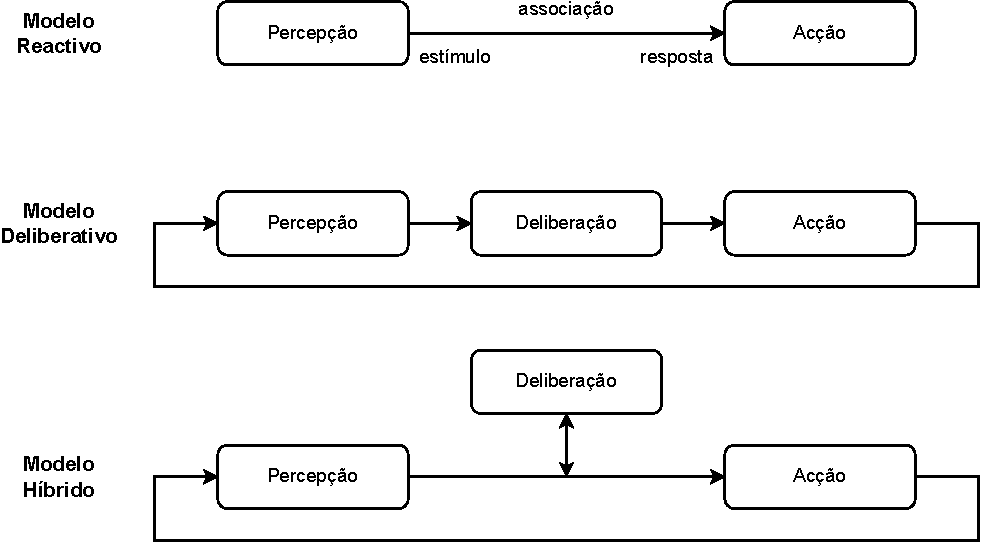
\includegraphics[scale=0.8]{modelos}
\caption{Diagramas dos 3 modelos usadas na arquitetura de agentes}
\end{figure}

\newpage
\paragraph{Arquitetura de Agentes Reactivos}
Neste tipo de arquitetura, o comportamento do sistema é gerado de forma reativa, baseando-se em associações entre estímulos. Os objetivos não estão representados de forma explicita, pelo contrário, encontram-se de forma implícita nas associações estímulo-resposta que definem o comportamento do agente.
Existe um acoplamento forte com o ambiente, em alguns casos directo, através de associações entre os estímulos derivados das percepções e a respostas que produzem acções.
Neste tipo de arquitetura, as acções são directamente activadas em função das percepções. Não são utilizadas representações internas do mundo, as respostas são rápidas mediante alterações no ambiente, e são fixas e predefinidas aos estímulos do ambiente, ou seja, para um mesmo estímulo, é sempre atuada a mesma acção.

No caso de reacções simples, as associações estímulo-resposta podem ser definidos através de regras SE-ENTÃO. Por exemplo, SE for avistado um animal, ENTÃO tirar fotografia.
No entanto, as reacções podem envolver processamentos mais complexos incluindo a manutenção de estado interno com base em mecanismos de memória. Nessa situação, os vários elementos envolvidos numa reacção devem ser modularizados, de forma a poderem ser organizados de forma versátil e a encapsular a complexidade necessária à sua função. Em particular, devem ser definidos os seguintes elementos:

\begin{description}
	\item[Estímulo] - Define informação activadora de uma reacção.
	\item[Resposta] - Define uma resposta a estímulos, em termos de acção a realizar e da respectiva prioridade.
	\item[Reacção] - Módulo que associa estímulos a respostas.
\end{description}

Nesta arquitetura, o agente reactivo é composto por conjuntos de reacções, as quais devem ser organizadas de forma modular em módulos comportamentais designados comportamentos, de modo a reduzir a complexidade e a facilitar o desenvolvimento e manutenção do agente. Um comportamento é um conjunto de reacções relacionadas entre si no sentido de produzirem um resultado específico, por exemplo, evitar um obstáculo.  Um comportamento realiza de forma modular e coesa o encapsulamento das reacções internas, contribuindo assim para reduzir o acoplamento e a complexidade da arquitectura de um agente reactivo.
Um comportamento pode também ser composto por outros comportamentos, tratando-se assim de um comportamento composto. Este tipo de comportamentos necessita de um mecanismo de selecção de acção para determinar a acção a realizar em função das respostas dos vários comportamentos internos.
Existem vários mecanismos de selecção, que podem executar acções em paralelo, escolher acções por prioridade, ou até combinar acções. Dois tipos de mecanismos de selecção de acção que escolhem uma acção por prioridade são: a hierarquia, e a prioridade.

\begin{description}
	\item[Hierarquia] - Os comportamentos estão organizados numa hierarquia fixa de subsunção (supressão e substituição)
	\item[Prioridade] - As respostas são seleccionadas de acordo com uma prioridade associada que varia ao longo da execução.
\end{description}

\begin{figure}[h]
\centering
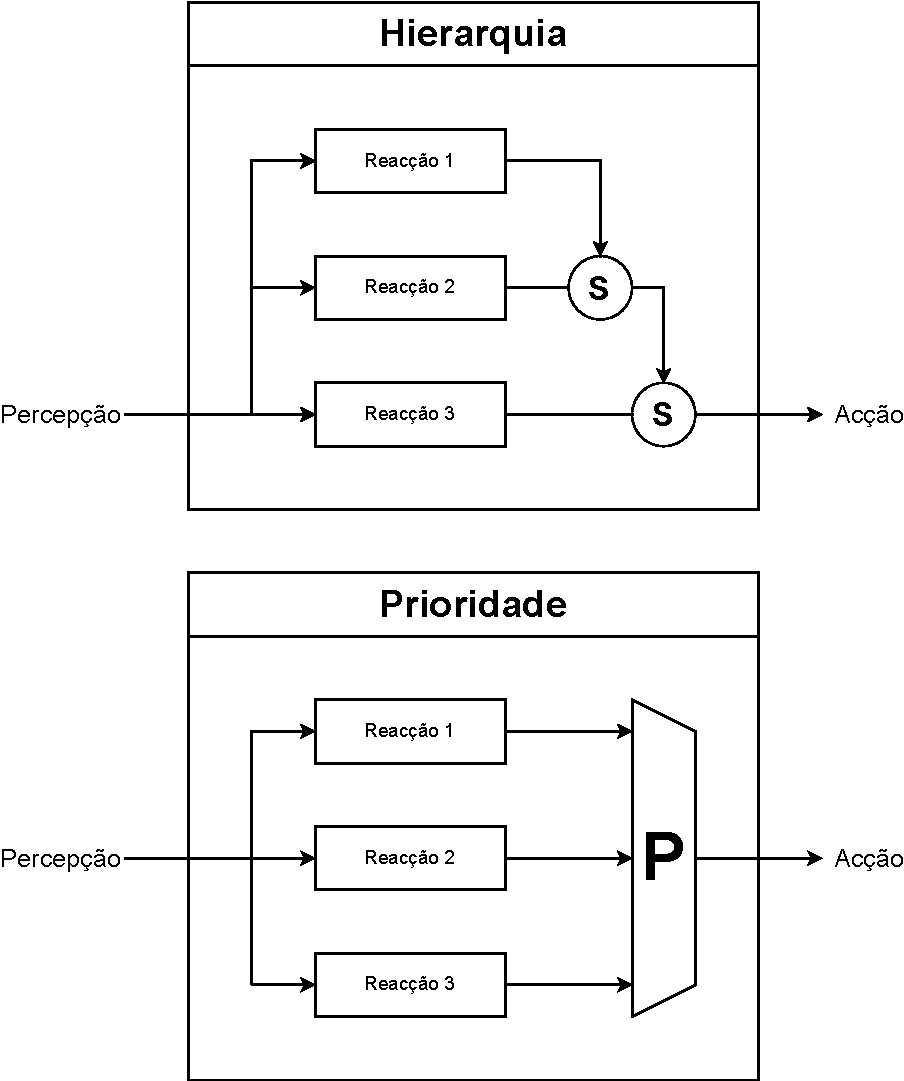
\includegraphics[scale=0.5]{mecanismosselecao}
\caption{Diagrama dos mecanismos de seleção: hierarquia e prioridade}
\end{figure}

Na concretização de uma arquitectura de agente, o processamento interno que relaciona percepções com acções, pode ser modularizado com base num módulo de controlo.
No caso da arquitectura de um agente reactivo, esse controlo será um controlo reactivo, em que o processar das percepções é realizado com base num módulo comportamental, também designado comportamento, o qual representa o comportamento geral do agente que pode ser constituído por diferentes sub-comportamentos.

Para modelação dos comportamentos de um agente reactivo, deve ser realizada a análise do domínio do problema a resolver para identificação de diferentes aspectos, como a informação que o agente recebe do ambiente (para modelação das percepções), que tipo de acções a realizar e, em particular, qual a finalidade do agente, definida em termos de objectivos concretos.
A concretização dos objectivos identificados, deve posteriormente ser modelada sob a forma de comportamentos, os quais, por sua vez, podem ser definidos em termos de sub-objectivos que serão realizados sob a forma de sub-comportamentos, de forma modular.

A arquitetura reativa pode ser implementada com memória, e nesse caso, as reacções para além de dependerem das percepções, dependem também da memoria de percepções anteriores para gerar as ações, as reacções podem envolver não apenas percepções, mas também estado interno (memória). As vantagens de manter o estado interno são:
\begin{itemize}
	\item pode produzir todo o tipo de comportamento.
	\item Pode representar dinâmicas temporais, evoluindo o estado, e a resposta ser definida tendo em conta percepções anteriores.
	\item Possibilidade de comportamentos mais complexos baseados na evolução de estado.
	\item Capacidade de lidar com situações de falha por exploração de acções não realizadas anteriormente.
\end{itemize}

Algumas desvantagens são:
\begin{itemize}
	\item Elevada complexidade espacial (memória).
	\item Elevada complexidade computacional (manter os estados).
	\item Mesmo com a manutenção de estado, as arquitecturas reactivas não suportam representações complexas, nem exploram planos alternativos de acção.
\end{itemize}

\paragraph{Arquitetura de Agentes Deliberativos}
Como foi anteriormente explorado, os agentes baseados em arquitecturas reactivas não são capazes de anticipar o futuro, sendo esta uma habilidade dos agentes deliberativos.

Numa arquitectura deliberativa, é a memória que desempenha o papel central na geração do comportamento do agente. É a memória que é o suporte de representação do mundo e dos mecanismos de deliberação, que são nomeadamente, mecanismos de raciocínio e de tomada de decisão.

Esta arquitectura o comportamento é gerado com base em processos de planeamento suportados pelo modelo do mundo.

Aplicando os conceitos do raciocínio automático ao conceito do agente autónomo, encontramos o raciocínio prático. Este tipo de raciocínio é orientado para a acção, e são utilizadas representações simbólicas dos objectivos a atingir, das acção que os agente pode realizar e do ambiente, sendo posteriormente gerados planos de acção que vão ditar o comportamento do agente.

Este tipo de raciocínio é caracterizado por 2 principais componentes, sendo estas: a deliberação, ou seja, o raciocínio sobre os fins a atingir, e que tem como resultado um conjunto de objectivos a concretizar, e o planeamento, ou seja, o raciocínio sobre as acções e recursos necessários para atingir os fins, que tem como resultado planos de acção para conseguir concretizar os objectivos determinados pela deliberação.

Estas duas componentes são suportadas pelo modelo do mundo, que é atualizado pelas percepções do ambiente, mas também por efeito de mecanismos de raciocínio prático, estes que também podem ser influenciados pelas percepções, em específico, através de eventos que influenciam os mecanismos de deliberação e planeamento.

Nestas arquiteturas, é o raciocínio prático que suporta o processo geral de tomada de decisão que determina o comportamento do agente, ou seja, quais as acções a realizar dadas as percepções obtidas e o estado do modelo do mundo.

O processo de tomada de decisão e acção tem os seguintes passos:
\begin{enumerate}
	\item Observar o mundo (mais concretamente, gerar percepções)
	\item Actualizar o modelo do mundo
	\item Se for não for necessário reconsiderar, saltar para o passo 6.
	\item Deliberar o que fazer (mais concretamente, gerar um conjunto de objectivos)
	\item Planear como o fazer (ou seja, gerar um plano de acção)
	\item Executar o plano de acção.
\end{enumerate}

Neste tipo de arquiteturas, o modelo do mundo e os mecanismos de raciocínio prático podem ser organizados num controlo deliberativo, que executa todo o processo de tomada de decisão e acção, recebendo percepções, e gerando acções.

\subsubsection{Processos de Decisão Sequencial}


\newpage
\subsection{Engenharia de Software em I.A.}
\subsubsection{O que é?}
A engenharia de software é uma área de engenharia orientada para a especificação, desenvolvimento e manutenção de software, que tem por objectivo o desenvolvimento, operação e manutenção de software de modo sistemático e quantificável.
\begin{description}
	\item[Sistemático] - Significa a capacidade de realizar o desenvolvimento de software de forma organizada e previsível, de modo a garantir a satisfação dos requisitos definidos, incluindo tempo e recursos necessários.
	\item[Quantificável] - Significa a capacidade de avaliar os meios envolvidos e os resultados produzidos no desenvolvimento de software, utilizando métodos e processos adequados para garantir a qualidade e o desempenho do software produzido, bem como a criação de documentação e a monitorização do processo de desenvolvimento.
\end{description}

O desenvolvimento de software de forma sistemática e quantificável é importante para garantir que os requisitos do software sejam cumpridos, bem como para prever e gerir os recursos necessários para o desenvolvimento e operação do software produzido.
Além disso, a aplicação das boas práticas da engenharia de software leva a software mais robusto e produzido com maior rapidez.

Existem dois principais obstáculos que crescem ao longo do desenvolvimento: a complexidade e a mudança.
\subsubsection{Complexidade}
Expressa na crescente dificuldade de desenvolvimento, operação e manutenção de software, na crescente sofisticação do software produzido, bem como na quantidade crescente de recursos envolvidos, nomeadamente, em termos de capacidade de processamento e de memória utilizada.

O crescimento da complexidade de um sistema de forma não adequadamente controlada, pode tornar o esforço de desenvolvimento muito elevado, a ponto de comprometer a viabilidade do respetivo projecto. Isto deve-se ao facto da complexidade crescer exponencialmente, ou seja, um sistema com duas vezes mais partes é muito mais do que duas vezes mais complexo.

Para melhor entender o nível de complexidade, é possível dividir a complexidade em dois tipos:
\begin{description}
	\item[Complexidade organizada] - Resulta de padrões de inter-relacionamento entre as partes correlacionáveis no espaço e no tempo. 
	\item[Complexidade desorganizada] - Resulta do número e heterogeneidade das partes de um sistema. As partes podem interagir entre si, mas a interacção é irregular.
\end{description}

\subsubsection{Mudança}
A mudança é expressa no ritmo crescente a que o software necessita de ser produzido, ou modificado, para satisfazer as necessidades dos respetivos contextos de utilização, quer a nível de funcionalidades disponibilizadas, quer a nível das tecnologias utilizadas.

\subsubsection{Arquitetura de Software}
A arquitectura de software tem por objectivo abordar o problema da complexidade com base numa organização adequada do software a produzir.
Para abordar este problema, necessitamos de 3 vertentes: métricas, princípios e padrões.

\subsubsection{Métricas}
Existem várias métricas para quantificar a qualidade da arquitetura:
\begin{description}
	\item[Acoplamento] - O conceito de acoplamento refere-se ao grau de dependência entre diferentes partes de um sistema, sendo tanto maior quanto maior a dependência entre as partes de um sistema. Pode ser medido utilizando diferentes métricas, como o número de associações entre elementos ou o grau de complexidade de uma interface. Quanto menor, melhor.
	\item[Coesão] - O conceito de coesão refere-se à forma como os elementos de um sistema estão agrupados de forma coerente entre si, será tanto maior quando mais relacionados entre si forem os elementos agrupados em cada módulo. Pode ser medida utilizando diferentes critérios, por exemplo, por tipo de função das partes agrupadas, sendo designada neste caso por coesão funcional. Quanto maior, melhor.
	\item[Simplicidade] - Nível de facilidade de compreensão/comunicação da arquitectura.
	\item[Adaptabilidade] - Nível de facilidade de alteração da arquitectura para incorporação de novos requisitos ou de alterações nos requisitos previamente definidos.
\end{description}
\subsubsection{Princípios}
\begin{description}
	\item[Abstração] - Ferramenta base para lidar com a complexidade, é o processo de descrição de conhecimento a diferentes níveis de detalhe e tipos de representação. Por exemplo, ao modular uma maçã e uma banana, é possivel abstrair conceitos comuns para um terceiro tipo, neste caso fruta, do qual ambos a maçã e a banana derivam/extendem.
	\item[Modularização] - O conceito de modularização refere-se à capacidade de organização de um sistema em partes coesas, ou módulos, que podem ser interligados entre si para produzir a função do sistema, está relacionado com dois aspectos principais, decomposição e encapsulamento.
		\begin{description}
			\item[Decomposição] - Partir um sistema em partes coesas. Por exemplo, dividir as representações de percepções e de acções em diferentes módulos.
			\item[Encapsulamento] - Isolamento dos detalhes interiores de parte do sistema para as restantes partes, permitindo o acesso apenas através da sua interface (contracto funcional).
		\end{description}
	\item[Factorização] - A decomposição das partes de um sistema de modo a eliminar redundância. Por exemplo, se duas funções partilham algum código, é possivel realizar uma terceira função que execute apenas o código comum, para que esse código esteja presente numa única função.
\end{description}

\subsubsection{Unified Modeling Language - UML}
O desenvolvimento de sistemas com base em inteligência artificial é caracterizado pela elevada complexidade desses sistemas. Como tal, requer métodos adequados de engenharia de software, nomeadamente, no que se
refere à modelação de sistemas, bem como a linguagens de modelação adequadas, como é o caso da linguagem UML.
	
\newpage
\section{Projecto – Parte 1}
A primeira parte do projeto trata-se de um agente reactivo, e de um ambiente sobre o qual este actua. Esta primeira parte foi desenvolvida em Java.
O agente reactivo encontra-se num jogo, com um ambiente virtual. O seu objectivo é fotografar os animais que conseguir encontrar.

Primeiro, foi desenvolvido o ambiente, comando e evento. O ambiente modulado é capaz de evoluir, observar um evento e executar um comando.
Tanto o ambiente, como o evento e comando tratam-se de interfaces, que tal como referido anteriormente, diminuem o acoplamento da arquitetura. O uso de interfaces é um bom exemplo de encapsulamento, visto que os detalhes da implementação são ocultados pelo contrato funcional (interface) que é definido.
Neste subsistema, é já possivel observar uma dependência, visto que Ambiente depende tanto de Evento como de Comando. A relação entre estas classes é apenas uma dependência, visto que o único uso é como parâmetro num método. Este tipo de relação é o tipo com menor acoplamento.

De seguida, foi então modulado o agente, o controlo, a percepção e a acção.
Neste subsistema, já é possivel ver um exemplo de uma associação (por exemplo, de Percepção para Evento), que tem maior acoplamento que uma dependência. Esta associação acontece visto que a percepção contém uma referência para um evento.
Também é possível observar uma composição (de Agente para Controlo), que tem ainda maior acoplamento que uma associação. A composição acontece quando uma parte é composta por outras parte que só existem no contexto da parte composto, neste caso, Agente é composto por Controlo, e um Controlo só existe no contexto de um Agente.
É também de notar que neste sistema existe também pela primeira vez a necessidade de existirem atributos \textit{read only} (apenas de leitura). Em Java, isto é possivel através do encapsulamento do atributo (ou seja, o atributo é privado e existem \textit{getters} e \textit{setters}, neste caso apenas existe o \textit{getter}, visto que é \textit{read only}).

De seguida foi modulado o subsistema do ambiente do jogo, modulando as classes AmbienteJogo, EventoJogo e ComandoJogo.
Neste subsistema, temos um exemplo de uma realização de uma interface (por exemplo, AmbienteJogo realiza Ambiente). Esta é a relação com maior acoplamento (juntamente com a generalização).
Neste caso específico, o ambiente do jogo evolui através da geração de novos eventos. Esta geração acontece através do \textit{input} do utilizador, podendo este escolher entre os eventos possiveis.

De seguida, foi modulado o subsistema da personagem, desenvolvendo a classe Personagem.
Neste subsistema, aparece finalmente uma generalização (de Personagem para Agente), que tal como foi referido anteriormente, é uma das relações com maior acoplamento.

De seguida, foi modulado o subsistema Jogo, que apenas incorpora a classe Jogo.
Esta classe tem o método main.

De seguida, foram moduladas as classes MaquinaEstados, Estado e Transição.

Para finalizar a primeira parte do projeto, foi então modulada a classe ControloPersonagem.

Após finalizadas todas as classes, foi possivel testar e concluir que o programa estava a funcionar corretamente, sem a necessidade de corrigir algum tipo de código. Isto foi apenas possivel graças à aplicação de boas práticas da engenharia de software durante o desenvolvimento do código, passando por exemplo, pelo desenvolvimento do código estrutural antes do desenvolvimento do código comportamental.

Estando concluída a primeira parte do projeto, foi então iniciada a segunda parte.

\newpage
\section{Projecto – Parte 2}
A segunda parte do projeto trata-se de uma biblioteca para o desenvolvimento de agentes reactivos (ecr), e da modulação de um agente para percorrer um ambiente, onde este deve recolher os alvos. Esta parte (e as seguintes) foi desenvolvida em Python.

Para esta parte do projeto (e para as seguintes partes também), foi utilizado o sae (Simulador de Ambiente de Execução), biblioteca que representa um ambiente. Esta foi fornecida pelo docente.

Dando inicio à segunda parte do projeto, começamos por desenvolver a biblioteca ecr.

Após o desenvolvimento da biblioteca, foi então desenvolvido o controlo reactivo, o comportamento Explorar, a resposta RespostaMover e a hierarquia Recolher.
Com estas classes desenvolvidas, foi possivel testar uma versão simples do agente, usando apenas o comportamento Explorar dentro da hierarquia Recolher. Foi verificado que o agente movia-se aleatoriamente, e que por vezes recolhia os alvos, como esperado.

De seguida, foram desenvolvidas as classes AproximarDir, EstimuloAlvo, AproximarAlvo, EvitarDir, EstimuloObst, EvitarObst e RespostaEvitar.
Com estas classes desenvolvidas, é agora possivel incluir não só o comportamento Explorar na hierarquia Recolher, como também os comportamentos AproximarAlvo e EvitarObst. Foi então testado a nova versão do agente, com os novos comportamentos, e verificado que este já não tentava avançar contra paredes, e que ia ao encontro dos alvos quando os percepcionava.

No final desta parte do projeto, e como foram também aplicadas as boas práticas da engenharia de software durante o desenvolvimento do código, foi apenas necessário corrigir no ControloReact, para que este mostrasse a informação sensorial.
Sendo verificado que o comportamento agora era o expectável, foi então dada como concluida a segunda parte do projeto.

\newpage
\section{Projecto – Parte 3}
Ainda não incluída.

\newpage
\section{Projecto – Parte 4}
Ainda não incluída.

\newpage
\section{Revisão do projecto realizado}
Durante as diversas entregas ocorreram poucos erros, sendo o mais notável a falta de documentação e justificação teórica para o código desenvolvido. Esta deve-se à diferença entre a documentação/justificação teórica (e a forma como esta é pedida, sobre a forma de comentários no código) nesta Unidade Curricular, com a documentação habitual entregue nas restantes unidades curriculares de LEIC (e mesmo quando é necessário algum tipo de justificação teórica, esta é entregue separadamente). De resto, as entregas foram entregues sem erros de código.

\newpage
\section{Conclusão}
O projeto até ao momento abordou vários tópicos fundamentais da Inteligência Artificial para Sistemas Autónomos e da Engenharia de Software, tais como os agentes reactivos e o desenvolvimento de codigo com suporte em UML.
Com a conclusão da parte 1 e 2 da unidade curricular, é possivel concluir que está desenvolvido, na teoria e prática, uma forte base para a aprendizagem dos seguintes tópicos da unidade curricular, tais como a procura em espaço de estados.

\newpage
\nocite{*}
\printbibliography[heading=bibintoc]

\end{document}